\section{Introduction}
First, we will look at the basic mathematical concepts that ultimately underpin the whole theory. So let's start with so-called meshes and look at some examples and how these mathematical concepts can be implemented in code using \maniflow{}.
\begin{defi}[Mesh]
    Let $V$ be a vector space  over $\R$ of dimension $n$. Let $\mathcal{V}_M\subset V$ be a set of points in $V$. We further let $\mathcal{F}_M\subset\mathcal{V}_M^3$. The pair $M = (\mathcal{V}_M, \mathcal{F}_M)$ is then called mesh. The elements of $\mathcal{V}_M$ are called points of $M$ and the elements of $\mathcal{F}_M$ are the faces of the mesh $M$.
\end{defi}
For a mesh $M = (\mathcal{V}_M, \mathcal{F}_M)$ we will often denote $V_M = \vert\mathcal{V}_M\vert$ and $F_M = \vert\mathcal{F}_M\vert$.
\paragraph{Remark.} Meshes $M$ can be considered as $2$-dimensional simplicial complexes. Thus for $2$-dimensional manifolds $\Tilde{M}\subset V$ we may find a \textit{triangulation} simplicial complex $K$ of $\Tilde{M}$. The corresponding mesh will be called \textit{triangulation} mesh of the manifold $\Tilde{M}$.
\begin{ex}[Tetrahedron]\label{ex:tetra} Let 
\begin{align*}
    \mathcal{V} = \left\{\left(\sqrt{\frac89},0,-\frac13\right),\left(-\sqrt{\frac29},\sqrt{\frac23},-\frac13\right),\left(-\sqrt{\frac29},-\sqrt{\frac23},-\frac13\right), \left(0,0,1\right)\right\}\subset\R^3
\end{align*}
and $\mathcal{F} = \{f\in2^{\mathcal{V}}:\vert f\vert = 3\}$. The mesh $T = (\mathcal{V},\mathcal{F})$ is the tetrahedron, which is displayed in figure \ref{fig:tetra}.
    \begin{figure}[h]
        \centering
        \includesvg[scale=0.6]{img/tetrahedron.svg}
        \caption{Tetrahedron}
        \label{fig:tetra}
    \end{figure}
This can be implemented using \texttt{maniflow} by using the \texttt{Mesh} class:
\begin{lstlisting}
import numpy as np
import itertools
from maniflow.mesh import Mesh, Face

# computing the four vertices of the tetrahedron
v1 = np.array([np.sqrt(8/9), 0, -1/3])
v2 = np.array([-np.sqrt(2/9), np.sqrt(2/3), -1/3])
v3 = np.array([-np.sqrt(2/9), -np.sqrt(2/3), -1/3])
v4 = np.array([0, 0, 1])

tetra = Mesh()
# setting the vertices as the vertices of the new mesh object
tetra.vertices = [v1, v2, v3, v4]
# now we compute the subsets of all the vertices consiting of three vertices
subsets = set(itertools.combinations(list(range(tetra.v)), 3))
# the faces are then set as the faces of tetra
tetra.faces = [Face(tetra, *list(i)) for i in subsets]
\end{lstlisting}
This way, we obtain the \texttt{Mesh} object \texttt{tetra} which represents a tetrahedron.
\end{ex}
\subsection{Reading and writing \texttt{.obj} files}\label{sec:objfiles}
The repeated computation of meshes can require a lot of computing capacity under certain circumstances. It can also be difficult to programme complicated geometries line by line in the code. To avoid these difficulties, \maniflow{} supports the \texttt{.obj} file format.
This makes it possible to export meshes for further editing in other programmes (e.g. \href{https://www.blender.org/}{Blender} or similar) or to display them\footnote{if you do not want to use the internal renderer of \maniflow{}}.
You can also use third-party software to create complicated geometries relatively easily and import them into \maniflow{}.
Interaction with .obj files is made possible by the maniflow.mesh.obj.OBJFile class.
\paragraph{Caution:} \texttt{maniflow.mesh.obj.OBJFile} currently disregards any normal vectors, texture coordinates, line elements etc. defined in the \texttt{.obj} file.
Only the coordinates of the vertices are taken into account and for the faces only the indices of the vertices that make them up are taken into consideration.
\begin{ex}
    Consider the \texttt{Mesh} object \texttt{tetra} from example \ref{ex:tetra}. To store this mesh in a \texttt{.obj} file, we may use
    \begin{lstlisting}
from maniflow.mesh.obj import OBJFile

OBJFile.write(tetra, "examples/tetrahedron.obj")
    \end{lstlisting}
    This code produces the file \url{examples/tetrahedron.obj}. In order to load a mesh into \maniflow{}, simply use
    \begin{lstlisting}
mesh = OBJFile.read("examples/tetrahedron.obj")
    \end{lstlisting}
\end{ex}
\subsection{\texttt{maniflow.mesh.utils.VertexFunction} -- Creating meshes from parameterisations}
The way we created a mesh of a tetrahedron in the previous example is very static and absolutely not suitable if you want to study more complicated geometries. \maniflow{}, however, provides the option of creating meshes quite easily using parameterisations. For this purpose, \maniflow{} provides the wrapper \texttt{maniflow.mesh.utils.VertexFunction}, which executes a given function on all vertices of the mesh and has the resulting mesh as output.
\begin{ex}
    For the following example, we assume that we have a \texttt{Mesh}-object \code{mesh} and we want to shift this mesh by the vector $\begin{pmatrix}1 & 2 & 3\end{pmatrix}^{\intercal}\in\R^3$. For this we make use of a \texttt{VertexFunction}:
    \begin{lstlisting}
# importing the wrapper from maniflow.mesh.utils
from maniflow.mesh.utils import VertexFunction

# implementing the VertexFuntion 'shift'
@VertexFuntion
def shift(vertex):
    return vertex + np.array([1, 2, 3])


# applying 'shift' to 'mesh'
shifted = shift(mesh)
    \end{lstlisting}
    The resulting \texttt{Mesh}, \code{shifted}, is \code{mesh} shifted by the vector $\begin{pmatrix}1 & 2 & 3\end{pmatrix}^{\intercal}\in\R^3$.
\end{ex}
Another application of this would be the creation of meshes from parameterisations $\psi\colon \R^2\supset D\to\R^3$. Oftentimes, the domain $D$ is a cartesian product of two intervals, so $D = I_1\times I_2$.\footnote{Or to be more precise, \maniflow{} makes it easy to create meshes from parametrisations, where the domain $D$ is homoeomorphic to a square.} For this, \maniflow{} provides the class \texttt{maniflow.mesh.parameterized.Grid}.
\begin{ex}[Moebius strip]\label{ex:moebius_creation}
We now turn to an example where we want to create a triangulation of a moebius strip. To this end, we will use the parametrisation
\begin{align*}
    \psi\colon [0, 2\pi]\times [-1,1]\to\R^3,\ (u,v)\mapsto\begin{pmatrix}
        \left(1+\frac{v}{2}\cos{\frac{u}{2}}\right)\cos{u}\\
        \left(1+\frac{v}{2}\cos{\frac{u}{2}}\right)\sin{u}\\
        \frac{v}{2}\sin{\frac{u}{2}}
    \end{pmatrix}.
\end{align*}
In order to discretise the set $[0,2\pi]\times[-1,1]$, we make use of \texttt{maniflow.mesh.parametrized.Grid} in order to create a high resolution lattice. Then we can implement a \texttt{VertexFunction} to capture the parametrisation $\psi$ in code and apply it to our lattice.
\begin{lstlisting}
from maniflow.mesh.parameterized import Grid
from maniflow.mesh.utils import VertexFunction


# implementing the parametrisation 1:1 in code as a VertexFunction
@VertexFunction
def moebius(vertex):
    x = vertex[0]
    y = vertex[1]
    x0 = np.cos(x) * (1 + (y / 2) * np.cos(x / 2))
    x1 = np.sin(x) * (1 + (y / 2) * np.cos(x / 2))
    x2 = (y / 2) * np.sin(x / 2)
    return np.array([x0, x1, x2])


u = Grid((0, 2 * np.pi), (-1, 1), 30, 10)  # create a high resolution grid
moebiusMesh = moebius(u)  # mapping the vertices from the grid according to the parametrisation
coincidingVertices(moebiusMesh) # remove the redundant vertices at the joint after making the moebius band
\end{lstlisting}
With this we obtain the \texttt{Mesh}-object \code{moebiusMesh}. Using \texttt{maniflow.mesh.obj.OBJFile}, we can write this mesh to memory as a \texttt{.obj} file, see section \ref{sec:objfiles}
\begin{lstlisting}
from maniflow.mesh.obj import OBJFile

OBJFile.write(moebiusMesh, "examples/moebius.obj")
\end{lstlisting}
Unsurprisingly, one can then load this file into \href{https://www.blender.org/}{Blender} and create pictures of it etc.\footnote{\maniflow{} comes with its own simple renderer. But if you want to do more elaborated computer graphics, you might consider using some other software to render images.} Figure \ref{fig:moubius_blender} shows a screenshot taken from Blender with the \texttt{.obj} file from \href{https://gitlab.gwdg.de/yangshan.xiang/scientific-computing/-/blob/82c42c864b3e46303b208b78720b8109116c78da/examples/moebius.obj}{\url{examples/moebius.obj}}.
\end{ex}
\begin{figure}[t]
    \centering
    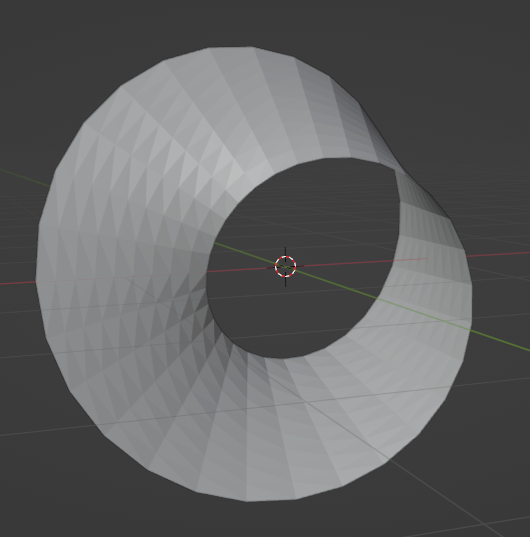
\includegraphics[scale=0.35]{img/moebius_2023-05-23.png}
    \caption{Screenshot of \href{https://www.blender.org/}{Blender} with a moebius strip made with \maniflow{}}
    \label{fig:moubius_blender}
\end{figure}
\newpage
